\documentclass{beamer} % [aspectratio=169]
\usetheme{ucl}
\setbeamercolor{banner}{bg=brightblue}
\setbeamersize{description width=2em}
\setbeamertemplate{navigation symbols}{\vspace{-2ex}} 


%\usepackage{fontspec}
\usepackage[utf8]{inputenc}
% \usepackage[english, greek]{babel}


\usepackage[T1]{fontenc} % Turn £ into $
\usepackage{minted}
\usemintedstyle{emacs}

\usepackage{fancyvrb}
\usepackage{xcolor}
\usepackage{url}

\usepackage{natbib}
\usepackage{bibentry}
\usepackage{url}


\usepackage{tikz}
\usetikzlibrary{positioning}
\usetikzlibrary{calc,shapes.multipart,chains,arrows}



\newcommand\emc[1]{\textcolor{brightblue}{\textbf{#1}}}

\AtBeginSection[]{
  \begin{frame}
  \vfill
  \centering
  \begin{beamercolorbox}[sep=8pt,center,shadow=true,rounded=true]{title}
    \usebeamerfont{title}\insertsectionhead\par%
  \end{beamercolorbox}
  \vfill
  \end{frame}
}

\author{Prof.\ George Danezis, University College London, UK}
\title{Dynamic Data Structures \& Objects Oriented Concepts.}
\subtitle{ENGS102P: Design and Professional Skills }
% \institute{}
\date{Term 1, 2017}


\begin{document}
\nobibliography*


\frame{
\titlepage
}

\begin{frame}
\frametitle{How are the python dynamic data types implemented?}

Dynamic data types are those, like \emc{list}, that can grow and shrink in the number of elements they contain. Others grow and shrink while maintaining some \emc{invariants}, such as being sorted.

\vspace{3mm}
But \emc{how can you implement} lists or other such datatypes?

\vspace{3mm}
\begin{block}{Understand how things work!}
Great computer scientists use the \emc{best available libraries and native types}, but understand how they work sufficiently to make \emc{informed decisions} about their applicability to problems. When they are not applicable they know how to \emc{build their own}.
\end{block}

\end{frame}

\begin{frame}
\frametitle{Aims for this topic}

\begin{itemize}
	\item Understand how \emc{dynamic data types are implemented} \\ under the hood -- only using \emc{fixed size} types.
	\item Explore in details how to implement \emc{linked lists}.
	\item Introduce \emc{Object Oriented Programming} \\ to make your own data types look and feel like native ones.
	\item Implement a data type that maintains a \emc{sorted multi-set} \\ of items using a tree.
	\item Discuss the native \emc{dictionary type} (\texttt{dict}).
	\item Introduce the concept of \emc{Machine learning}, \\ and implement a decision forest for a task.
\end{itemize}

\end{frame}


\section{Defining your own data types}

\begin{frame}
\frametitle{The linked list data type.}

A \emc{linked list} is a container data type representing a \emc{sequence} of items. 

\begin{center}
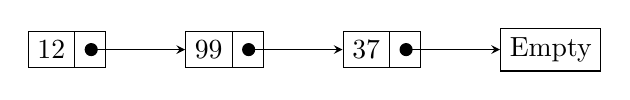
\begin{tikzpicture}[list/.style={rectangle split, rectangle split parts=2,
    draw, rectangle split horizontal}, >=stealth, start chain]

  \node[list,on chain] (A) {12};
  \node[list,on chain] (B) {99};
  \node[list,on chain] (C) {37};
  \node[on chain,draw] (D) {Empty};
  %\draw (D.north east) -- (D.south west);
  %\draw (D.north west) -- (D.south east);
  \draw[*->] let \p1 = (A.two), \p2 = (A.center) in (\x1,\y2) -- (B);
  \draw[*->] let \p1 = (B.two), \p2 = (B.center) in (\x1,\y2) -- (C);
  \draw[*->] let \p1 = (C.two), \p2 = (C.center) in (\x1,\y2) -- (D);
\end{tikzpicture}
\end{center}

\begin{itemize}
\item It is composed of a sequence of \emc{fixed size} `cells'. 
\item Each containing a \emc{head} item, and \emc{tail} pointing to the next cell.
\item The final cell points to a special cell representing the \emc{empty} list.
\end{itemize}

\begin{block}{Why focus on fixed-size cells to build dynamic data types?}
Operating systems implement allocators to provide programs with fixed areas of memory -- through costly allocations and de-allocation operations. Therefore we have to build dynamic data types (that will require more or less memory as they grow and shrink) from those units.
\end{block}
\end{frame}


\begin{frame}
\frametitle{Representing a linked list as tuples in Python.}

We will implement a linked list in Python, using \texttt{tuple} and \texttt{None}.
\begin{itemize}
\item We represent an empty linked list as the value \texttt{None}.
\item We represent a cell of a linked list as a tuple of \texttt{(head, tail)}.
\end{itemize}

\vspace{3mm}
We represent the linked list of values 12, 99 and 37 as:

\begin{center}
\texttt{(12, (99, (37, None)))}
\end{center}

\end{frame}


\begin{frame}
\frametitle{Linked list operations in Python.}

Simple algorithms on linked lists:
\begin{description}
  \item[empty()] --- returns an empty linked list (\texttt{None}).
  \item[cons(lList, item)] --- returns a list with item appended to lList.
  \item[head(lList)] --- returns the head item of the linked list.
  \item[tail(lList)] --- returns the tail linked list.
\end{description}

\vspace{3mm}
\begin{block}{Abstract interface to the linked list.}
By writing linked list algorithms to only use this restricted list of functions we can abstract the details of how linked lists are implemented. We are free to change this representation without modifying the algorithms. Such a set of functions is called an \emc{interface}.
\end{block}

\end{frame}

\begin{frame}
\frametitle{Linked list operations in Python.}

  \inputminted[
    firstline=3,
    lastline=17,
    xleftmargin=1.4em,
    frame=lines,
    framesep=2mm,
    %baselinestretch=1.2,
    % bgcolor=lightgray,
    fontsize=\footnotesize,
    linenos
  ]{python}{src/LinkedList.py}

All operations have time complexity $\mathcal{O}(1)$.


\end{frame}


\begin{frame}
\frametitle{Algorithms on linked list.}

More complex algorithms can be implemented in terms of the simpler algorithms:
\begin{description}
  \item[length(lList)] --- returns the number of items in the list.
  \item[index(lList, position)] --- returns the item at index `position' in the list, or throws an exception if it does not exist.
  \item[append(lList1, lList2)] --- returns a linked list with all elements of lList1 and lList2 in sequence.
  \item[isin(lList, item)] --- returns \texttt{True} if item is in the linked list.
  \item[Equals(lList1, lList2)] --- returns whether the lists contain exactly the same items.
\end{description}

\end{frame}

\begin{frame}
\frametitle{The length of a linked list.}

A recursive implementation to get the length of the list. Note that the equality is equivalent to a test on whether the list is empty. 

  \inputminted[
    firstline=19,
    lastline=24,
    xleftmargin=1.4em,
    frame=lines,
    framesep=2mm,
    %baselinestretch=1.2,
    % bgcolor=lightgray,
    fontsize=\footnotesize,
    linenos
  ]{python}{src/LinkedList.py}

Time complexity $\mathcal{O}(N)$ in $N$ the length of the list.

\end{frame}

\begin{frame}
\frametitle{Indexing a linked list.}

A recursive implementation of `index', to get the element position from the linked list.

  \inputminted[
    firstline=26,
    lastline=35,
    xleftmargin=1.4em,
    frame=lines,
    framesep=2mm,
    %baselinestretch=1.2,
    % bgcolor=lightgray,
    fontsize=\footnotesize,
    linenos
  ]{python}{src/LinkedList.py}

Time complexity $\mathcal{O}(N)$ in $N$ the length of the list.

\end{frame}

\begin{frame}
\frametitle{Appending two linked lists.}

A recursive implementation of appending two lists together. 

  \inputminted[
    firstline=37,
    lastline=42,
    xleftmargin=1.4em,
    frame=lines,
    framesep=2mm,
    %baselinestretch=1.2,
    % bgcolor=lightgray,
    fontsize=\footnotesize,
    linenos
  ]{python}{src/LinkedList.py}


\begin{block}{Leveraging immutability}
Note that all operations and algorithms never mutate linked lists, but instead return new ones. we leverage this in `append', to directly returns the second list once no more elements of the first one remain (line 40). If they were mutable, we would have to return a copy.
\end{block}

\end{frame}

\begin{frame}
\frametitle{Testing inclusion of an item in a linked list.}

A recursive implementation of `isin'.

  \inputminted[
    firstline=44,
    lastline=51,
    xleftmargin=1.4em,
    frame=lines,
    framesep=2mm,
    %baselinestretch=1.2,
    % bgcolor=lightgray,
    fontsize=\footnotesize,
    linenos
  ]{python}{src/LinkedList.py}

\end{frame}




\begin{frame}
\frametitle{Testing linked lists and operations.}

  \inputminted[
    firstline=53,
    lastline=68,
    xleftmargin=1.4em,
    frame=lines,
    framesep=2mm,
    %baselinestretch=1.2,
    % bgcolor=lightgray,
    fontsize=\footnotesize,
    linenos
  ]{python}{src/LinkedList.py}

\end{frame}


\begin{frame}
\frametitle{The structure of the linked list code.}

\emc{Patterns} and \emc{sources of error} in the linked list implementation:
\begin{itemize}
  \item Every operation and function takes a \emc{linked list as a first parameter}, aside from the constructor `empty'.
  \item The operation `equals' works due to the nature of the \emc{internal representation}. Those are visible to the programmer.
  \item Nothing prevents a careless programmer from passing an \emc{invalid} linked list.
  \item Validating list inputs would take $\mathcal{O}(N)$.
\end{itemize}

Could we protect the representation of the linked list, and ensure using the type system that linked lists are valid when operating on them?

\end{frame}

\section{Object Oriented Programming}

\begin{frame}
\frametitle{Objects = Data + Algorithms.}

Programming practice and style has to support a number of principles, we have explored already:

\begin{itemize}
  \item \emc{Classes}. Classes define \emc{custom types}, the \emc{operations permitted} on the type, and their  internal \emc{data representations}.
  \item \emc{Objects}. Objects are instances of a class and contain the data representing a custom type.
  \item \emc{Abstraction} \& \emc{Encapsulation}. No need to know the internal working of type to use them.
  \item \emc{Generics} \& \emc{Polymorphism}. We may use data types supporting similar operations to implement generic algorithms. 
  \item \emc{Inheritance}. Classes may inherit from others, to re-use code (do not over rely on this mechanism.)
\end{itemize}

\end{frame}


\begin{frame}
\frametitle{Classes, objects / instances and method syntax.}

  \inputminted[
    firstline=1,
    lastline=17,
    xleftmargin=1.4em,
    frame=lines,
    framesep=2mm,
    %baselinestretch=1.2,
    % bgcolor=lightgray,
    fontsize=\footnotesize,
    linenos
  ]{python}{src/toyclass.py}


\end{frame}

\begin{frame}
\frametitle{The Class LinkedList.}

  \inputminted[
    firstline=3,
    lastline=22,
    xleftmargin=1.4em,
    frame=lines,
    framesep=2mm,
    %baselinestretch=1.2,
    % bgcolor=lightgray,
    fontsize=\scriptsize,
    linenos
  ]{python}{src/LinkedListClass.py}


\end{frame}

\begin{frame}
\frametitle{Illustration of Encapsulation and Hiding.}

The implementation refactors linked list functions into a class.
\begin{itemize}
  \item Note that \texttt{\_representation} represents the internal state of the object.
  \item The underscore denotes that it should not be accessed directly as an attribute from outside the class definition.
  \item The method `cons', defined inside the class, directly manipulates this representation.
\end{itemize}

\end{frame}


\begin{frame}
\frametitle{Some algorithms as methods.}

Note we do not use the representation, even within the class.
  \inputminted[
    firstline=27,
    lastline=43,
    xleftmargin=1.4em,
    frame=lines,
    framesep=2mm,
    %baselinestretch=1.2,
    % bgcolor=lightgray,
    fontsize=\scriptsize,
    linenos
  ]{python}{src/LinkedListClass.py}


\end{frame}


\begin{frame}
\frametitle{The importance of immutability.}

We implement `append' by linking the tail of a new list to the other list directly, without first copying the other list.
  \inputminted[
    firstline=45,
    lastline=52,
    xleftmargin=1.4em,
    frame=lines,
    framesep=2mm,
    %baselinestretch=1.2,
    % bgcolor=lightgray,
    fontsize=\footnotesize,
    linenos
  ]{python}{src/LinkedListClass.py}


\end{frame}

\begin{frame}
\frametitle{Testing the LinkedList class.}

  \inputminted[
    firstline=120,
    lastline=139,
    xleftmargin=1.4em,
    frame=lines,
    framesep=2mm,
    %baselinestretch=1.2,
    % bgcolor=lightgray,
    fontsize=\scriptsize,
    linenos
  ]{python}{src/LinkedListClass.py}

\end{frame}


\begin{frame}
\frametitle{Overloading operators for seamless coding.}

How could we make our data type \texttt{LinkedList} behave like a native one?
  \inputminted[
    firstline=144,
    lastline=159,
    xleftmargin=1.4em,
    frame=lines,
    framesep=2mm,
    %baselinestretch=1.2,
    % bgcolor=lightgray,
    fontsize=\scriptsize,
    linenos
  ]{python}{src/LinkedListClass.py}


\end{frame}

\begin{frame}
\frametitle{Operators are represented by spacial methods.}

How could we make our data type \texttt{LinkedList} behave like a native one?
  \inputminted[
    firstline=82,
    lastline=98,
    xleftmargin=1.4em,
    frame=lines,
    framesep=2mm,
    %baselinestretch=1.2,
    % bgcolor=lightgray,
    fontsize=\scriptsize,
    linenos
  ]{python}{src/LinkedListClass.py}


\end{frame}



\begin{frame}
\frametitle{Iterators.}

Using the \texttt{yield} keyword returns the result, and `freezes' the state of the function as a \emc{generator}. Calling 'next()' continues from that point on. This allows us to implement \emc{iterators} easily:

\inputminted[
    firstline=106,
    lastline=112,
    xleftmargin=1.4em,
    frame=lines,
    framesep=2mm,
    %baselinestretch=1.2,
    % bgcolor=lightgray,
    fontsize=\scriptsize,
    linenos
  ]{python}{src/LinkedListClass.py}

Allowing the use of the object in a \texttt{for} loop:

\inputminted[
    firstline=158,
    lastline=159,
    xleftmargin=1.4em,
    frame=lines,
    framesep=2mm,
    %baselinestretch=1.2,
    % bgcolor=lightgray,
    fontsize=\scriptsize,
    linenos
  ]{python}{src/LinkedListClass.py}


\end{frame}

\section{Keeping a multi-set sorted.}

\begin{frame}
\frametitle{Motivation: keeping indexes for dynamic data structures.}

\begin{iterate}
  \item Searching is faster in sorted structures. Binary search is $\mathcal{O}(\log N)$.
\end{iterate}

\end{frame}

\begin{frame}
\frametitle{Trees and sorted trees.}
\end{frame}

\begin{frame}
\frametitle{Trees as branches and Leaves.}
\end{frame}

\begin{frame}
\frametitle{The TreeNode Class.}
\end{frame}

\begin{frame}
\frametitle{Adding items.}
\end{frame}

\begin{frame}
\frametitle{Removing items.}
\end{frame}

\begin{frame}
\frametitle{Searching.}
\end{frame}

\begin{frame}
\frametitle{Traversing in order.}
\end{frame}

\begin{frame}
\frametitle{Computational complexity.}
\end{frame}

\section{The Python \texttt{dict} type.}

\section{From programming to learning.}

\section{Ethics, Machine Learning and Artificial Intelligence.}

% ---------------------------------

\bibliographystyle{alpha}
\nobibliography{references}

\end{document}